% This file demonstrates how to use the IEEEConf LaTeX2e macro package,
% to prepare a manuscript for proceedings on CD of the conference
% FedCSIS
%
\documentclass[conference]{IEEEtran}

\IEEEoverridecommandlockouts

% This package serves to balance the column lengths on the last page of the document.
\usepackage{pbalance}

%% to enable \thank command
\IEEEoverridecommandlockouts
% to typeset algorithms
\usepackage{algorithmic}
\usepackage{algorithm}
% to make an accent \k be available
\usepackage[OT4,T1]{fontenc}
% provides various features to facilitate writing math formulas and to improve the typographical quality of their output.
\usepackage[cmex10]{amsmath}
\interdisplaylinepenalty=2500
% por urls typesetting and breaking
\usepackage{url}
% for vertical merging table cells
\usepackage{multirow}
\usepackage{flushend}

% define environments for remarks and examples
\newtheorem{remark}{Remark}[section]
\newtheorem{example}[remark]{Example}



\usepackage{booktabs}   %% For formal tables:
                        %% http://ctan.org/pkg/booktabs
\usepackage{subcaption} %% For complex figures with subfigures/subcaptions
                        %% http://ctan.org/pkg/subcaption
\usepackage{graphicx}
\usepackage{listings}
\lstset{basicstyle=\footnotesize\ttfamily,breaklines=true}
\lstset{framextopmargin=50pt,frame=bottomline}
\bibliographystyle{acm}

\begin{document}

\title{Compilation through interpretation}

\author{
	\IEEEauthorblockN{Adam Grabski}
	\IEEEauthorblockA{0000-0002-6283-8461\\
		Warsaw Univeristy of Technology\\
		in Warsaw\\
		ul.\ Nowowiejska 15/19, 00-665 Warsaw, Poland\\
		Email: adam.gr@outlook.com}
	\and
	\IEEEauthorblockN{Ilona Bluemke}
	\IEEEauthorblockA{0000-0002-2894-5976\\
		Warsaw Univeristy of Technology\\
		in Warsaw\\
		ul.\ Nowowiejska 15/19, 00-665 Warsaw, Poland\\
		Email: Ilona.Bluemke@pw.edu.pl}
}




%% \maketitle
%% Note: \maketitle command must come after title commands, author
%% commands, abstract environment, Computing Classification System
%% environment and commands, and keywords command.
\maketitle


\section{Introduction}

Compile-time function execution is an aspect of a programming language, that allows the programmer to execute code at compile-time.
The goals and capabilities of CTFE depend on the language and is discussed in chapter \ref{related-work}, however it plays a secondary role in the compilation process.

CTFE first builds the compiler around the interpreter component.
The role of the compiler is to construct the semantic model of the program being compiled and pass it as data to the interpreted Compiler-Intreface module.
Compiler-Interface then tranforms the model into the backend's assembly language to be compiled to executable.
The design of the language that sparked this approach was described in chapter \ref{language-design}.
Chapter \ref{compiler-design} deals with structure of a CTFE First compiler and how its components interact.

Using CTFE First approach carries with it certain unique implementation considerations.
Data structures used within the compiler and the way that the program is modeled is tightly coupled with the compiled language.
These challenges, as well as how they were solved in C-=-1 compiler were described in chapter \ref{implementation}.


\section{Related work}
\label{related-work}

Many currently used programming languages allow the programmer to execute some code at compile time, including C\# \cite{csharp:source_generators,roslyn}, Rust \cite{rust, klabnik2019rust} and C++ \cite{ISO:cpp20}.

Rust language compiler is the most similar in capability, to what was demonstrated with C-=-1, as a feature of CTFE First.
It allows the user to write code that performs some transformations of the program, and interact with the envoirment during the build process.
The two relevant features are build scripts and macros.

Rust macros, much like the classic C-style preprocessor macros, generate additional code as text.
The major difference between the systems is that Rust macros operate on tokens rather than text and use syntax similar to regular Rust code.
This mechanism is powerfull, allowing the user to rewrite code to avoid repetition, simplify certain tasks and create new syntax.
They are however unable to reflect on the program as a whole or obtain much of the information available to the compiler.

Build scripts, on the other hand, are programs that execute prior to compilation of the main package.
They prepare the envoirment for building the program by, for example, compiling its external dependencies.
They do not have any information about the structure of the program being compiled.
Build scripts that require such data, would have to analyze the code by itself, without any help from the compiler.
This makes application such as automatically genertaing bindings for other programming languages significantly more difficult.


\section{Design of C-=-1}
\label{language-design}

C-=-1 was designed as a compiled, low-level, non-garbage-collected programming language, similar to C, C++ or Rust.
What diffirentiates C-=-1 are its two founding principles: all code is executable at compile-time and support rich metaprogramming.
The primary purpose of the language was to research how these ideas influence software written in it \cite{grabski2022compilation}.

C-=-1 is a simple language, built with the minimum set of features needed to demonstrate the usefulness of the proposed metaprogramming features.
They are discussed further in chapter \ref{design:attributes_and_metaprogramming}.
The primary motivation for those mechanisms, is providing the programmer with the ability to create domain specific static analysis and code generation tools, without creating a seperate program.

\subsection{Type system}

C-=-1 type system heavily borrows from C++.
Program may contain user defined classes, with members which may have limited accessibility.
Generic programming is achieved by the use of templates, although they are mutch more limited than the ones present in C++.
The user may also use pointers to objects, with arbitrary indirection (for example pointer to pointer to object).
Additionally, the language contains the concept of an \lstinline{interface}, similar to the one found in C\#.

\subsection{Attributes and metaprogramming}
\label{design:attributes_and_metaprogramming}

Metaprogramming in C-=-1 is based around attributes.
Attributes work in a manner similar to the ones found in C\#.
They are types, which may contain fields and methods.
They can also, be used to annotate other elements of the program, such as types, functions or variables.

In C-=-1 these attributes may implement special member functions that react to uses of the annotated program element.
For example, an attribute that can be attached to a function, may implement \lstinline{onCall} special member function.
It will be called, at compile time, for each invocation of the annotated procedure.
Within the special method, the attribute will have access to the semantic model of the call site.
It may then modify the semantic model or report warnings or errors.

\begin{minipage}{\linewidth}

	\begin{lstlisting}[
	  numbers=left,
	  firstnumber=0,
	  caption={noDiscard attribute in C-=-1},
	  aboveskip=0pt,
	  label={lst:noDiscardCm1}
	  ]
  public att<function> NoDiscard
  {
	public fn attach(f: functionDescriptor)
	{}
	public fn onCall(call: functionCallExpression*)
	{
	if(call._parentStatment != null<IInstruction>())
	  raiseError(
		&(call._pointerToSource),
		"Return value of a no-discard function is not used",
		123
	  );
	}
  }
  \end{lstlisting}
\end{minipage}

Listing \ref{lst:noDiscardCm1} contains an example of a C-=-1 attribute: \lstinline{noDiscard}.
It works in the same manner as the attribute of the same name present in C++17 \cite{ISO:cpp17}: if applied to a function, the result of that invoking procedure must be used.

To declare an attribute in C-=-1, the \lstinline{att} keyword is used.
After that, attribute targets should be listed in angled brackets, as on line 0 of Listing \ref{lst:noDiscardCm1}.
Attributes may target any number of language elements, including types, functions, variables and fields.
Attribute from Listing \ref{lst:noDiscardCm1} declares two member functions: \lstinline{attach} on line 4 and \lstinline{onCall} on line 6.

The \lstinline{attach} method is called after names of all of the program elements have been gathered, but before the compiler started to analyze function bodies.
It is common accross all attribute targets and accepts the descriptor of the attached program element (function, field, type, etc.).
Only during call to \lstinline{attach} can the attribute change aspects of the program that affect function overload resolution, for example
whether a function is invokable at run or compile time.

The \lstinline{onCall} method is an example of a function reacting to usage of the annotated program element.
They are speciffic to a given attribute target.
Within this function, the attribute may analyze and modify the code, as well as raise errors or warnings.

Lines 6 to 11 of Listing \ref{lst:noDiscardCm1} are an example of a C-=-1 attribute providing static analysis.
The \lstinline{onCall} method checks whether the attached function is invoked in an expression or instruction context.
Calling a function as a statment means that the result of that invocation is discarded by the caller.
This is may indicate an error, when the function has no other side effects.
If that is the case, the attribute calls the \lstinline{raiseError} function, which is provided as a compiler intrinsic, that generates a compilation error.
The example presented in Listing \ref{lst:noDiscardCm1}, although very basic, demonstrates the ability to implement a form of static analysis that typically requires modyfining the compiler or creating an external tool.

\begin{minipage}{\linewidth}

	\begin{lstlisting}[
	  numbers=left,
	  firstnumber=0,
	  caption={Example of using noDiscard attribute from Listing \ref{lst:noDiscardCm1}},
	  aboveskip=0pt,
	  label={lst:noDiscardUsageCm1}
	  ]
  [noDiscard()]
  fn noDiscardFunction() -> usize;

  fn main() -> usize
  {
	noDiscardFunction();
	// error 123: Return value of
	// a no-discard function is not used
	let x = noDiscardFunction();     // ok
	let y = x + noDiscardFunction(); // ok
	return noDiscardFunction();      // ok
  }
  \end{lstlisting}
\end{minipage}

\section{Design of the compiler}
\label{compiler-design}

CTFE First apporach was created during implementation of the first compiler for the C-=-1 language\cite{grabski2022compilation}.
CTFE First compiler has four major components: Frontend, Interpreter, Compiler Interface and Backend.
Figure \ref{CTFE-first-compiler-structure} contains a diagram with an overview of how these parts interact with eachother, during the compilaton process.
Frontend, described in chapter \ref{frontend}, parses the code in the compiled language and constructs its intermidaite representation, using interpreter's data structures.
It is used to analyze both user code and the Compiler Interface.
After the intermidiate representation is constructed, it is passed on to the Interpreter, which was described in chapter \ref{interpreter}.
Compiler Interface intermidiate representation is then executed, using the user program as data.
This step converts the semantic model of the program into the backends intermidiate language.
This process is further explained in chapter \ref{compiler-interface}.
Finaly the Backend generates the executable file.

\begin{figure}
	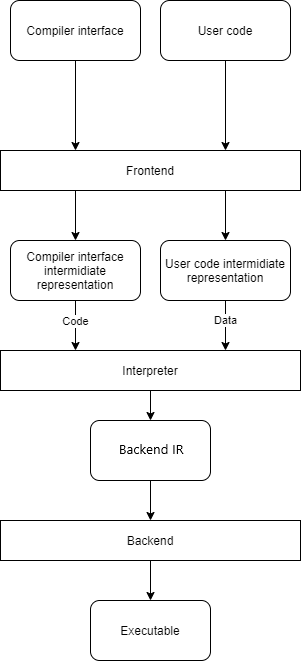
\includegraphics[height=10cm]{pictures/compiler-structure.png}
	\caption{CTFE First compiler structure}
	\label{CTFE-first-compiler-structure}
\end{figure}

\subsection{Frontend}
\label{frontend}

In the CTFE First approach, frontend serves the same role of constructing the programs intermidiate representation, as in conventional compilers \cite{puntambekar:compiler_design}.
The major difference lays in the data structures used to represent the program.

\subsection{Interpreter}
\label{interpreter}

In CTFE First, interpreter is the heart of the compiler.
It executes the Compiler-Interface which translates the intermidiate representation into the backend's assembly and serves as what is sometimes called the 'middle-end' of the compiler\cite{hsu2021llvm}.
To do it, it must be able to treat the program's intermidiate representation both as code and data.

An important consideration with implementing a CTFE First compiler, is what limitations to put on modifications of user code.
Depending on language design, it may be possible to introduce circular references between the functions that modify the codebase.
For example if function \lstinline{A} is modified by function \lstinline{B} and \lstinline{B} invokes \lstinline{A}, the behaviour of the program is unpredictable.
This problem will only be magnified by larger program sizes.

One of the possible solutions to the above mentioned problem is to limit which functions can be invoked at compiletime.
C-=-1 allows code within a compiletime context to invoke procedures only from other packages, declared explicitly as dependencies.
It additionally prohibits modification of dependencies.
Therefore its is impossible for a function to modify a procedure it depends on.% todo: wording, example

\subsection{Compiler Interface}
\label{compiler-interface}

Compiler Interface translates the program's intermidaite representation into the backend's assembly language.
This component is interpreted during compilation.
What is unique about CTFE First is that this part of the compiler can thus be written in the target language, during Stage 0 of the compiler bootstrapping process, as was the case for the C-=-1 compiler\cite{puntambekar:compiler_design, novillo2007gcc, grabski2022compilation}.

Compiler Interface is a regular code package that contains a function marked as the Compiler Interface Entry-point.
That procedure must accept a set of modules to be compiled and a Compilation Context that is used to generate the Backends assembly.
The module descriptors that are passed to the Compiler Interface are built by the frontend, as can be seen in figure \ref{CTFE-first-compiler-structure}.

After the Compiler Interface has finished generating backend assembly, the Compiler Backend is invoked to generate the binary executable.
\subsection{Backend}
\label{backend}

CTFE First does not put any additional requirements on compiler backend.
When using this pattern, an out-of-the-box backend library, can be used, as was the case with C-=-1 compiler.

The backend code must be invokable from within the interpreted program in the target language.
Depending on how the interpreter was designed, this can represent a significant undertaking.
Compiler backends are large and for the Compiler Interface to take advantage of them, they must be fully available.
This means exposing each function and type within the library, to the interpreted code.
These bindings could feasibly be generated automatically \cite{marshalling_auto_generation}, but this tehnique was not used when implementing C-=-1 compiler.


\section{Implementation}
\label{implementation}

The first CTFE First was created for the C-=-1 language, using out-of-the-box parser generator and backend.
The most important aspect of implementing a CTFE First compiler is the design of the data structures, described in chapter \ref{data_structures}, that will be used by the interpreter.

Languages that seek to exploit CTFE First approach in design of their compilers, should define a set of data structures to describe user code, i.e. a Semantic Model. %todo: languages are not people
It will allow the programmer to interact and mainpulate the structure of the program at compile-time.
The Semantic model designed and implemented for C-=-1 is described in chapter \ref{semantic_model}.

The final part of a CTFE First compiler is the Backend Interface.
It is a program, written in the target language, and ran at compile-time that translates the semantic model into the backends assembly language.
Backend Interface implemented for C-=-1 is relativley small and is described in chapter \ref{implementation/backend-interface}.

\subsection{Interpreter data structures}
\label{data_structures}
Data structures of the C-=-1 Interpreter have been designed ease of development and debugging in mind.
They are thus not particularly efficent.

\begin{figure}
	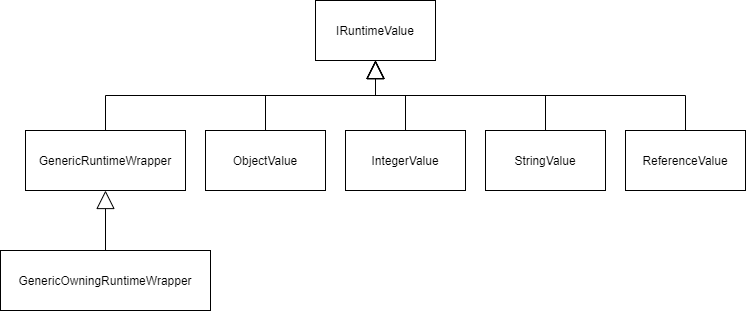
\includegraphics[width=8cm]{pictures/interpreter_data_structures_uml.png}
	\caption{Class diagram of C-=-1 interpreter data structures}
	\label{fig:interpreter_data_structures}
\end{figure}

Figure \ref{fig:interpreter_data_structures} contains a class diagram of most of the types used to represent values within C-=-1.
All of them derive from \lstinline{IRuntimeValue} and are managed via C++ smart pointers.
The interface of the base class allows the value to be converted to a human readable format, serialisation, deserialisation and copying.

The most primitive types within the hierarchy are \lstinline{StringValue} and \lstinline{IntegerValue}.
They are simple wrappers for strings and integers, present in the host language.
Floating point numbers were not implemented as they were not nessecary for implementation of a basic compiler.

User-defined types are represented using \lstinline{ObjectValue}.
The contents of an objects is kept as a \lstinline{string} - \lstinline{IRuntimeValue} dictionary, with field names as keys and \lstinline{uniqe_ptr<IRuntimeValue>} as values.
C-=-1 object is therefore spread out in memory, even if the fields are directly contained within the class, without any indirection.


There are multiple types of reference within the C-=-1 interpreter.
The most basic pointer type is a reference to C-=-1 value.
It was realised as a pointer to the owning pointer of the value.
The reasoning behind this decision was to allow assigning to the referenced value.

\subsection{Program semantic model}
\label{semantic_model}

A major motivation in creating CTFE First was the ability to support languages with compile-time metaprogramming.
This includes reflection and modification of the code being compiled.
User program has to be represented as a complete and modifiable object, using the interpreters data structures.

C-=-1 language model divides the user program into assemblies.
They represent an individual program package: a library or an executable file.
The compiler is invoked to compile an assembly, together with its dependencies.
Assembly is the root object of C-=-1 program model, it stores a list of assemblies it depends on and the root namespace of the package it represents.
The remainder of user code is organised around namespaces, types, functions and fields.
These parts of the model are repesented by native classes of the host language and form the basis for the rest of the model.

The most complex part of the model is the representation of the function body.
Like in most programming languages, a C-=-1 function can contain a variety of instruction types.
That includes complex statements and blocks of statements that can be arbitrarly nested.
Each instruction may also contain expressions of any complexity.

To deal with this complexity, C-=-1 semantic model for functions is build around two interfaces: \lstinline{IInstruction} and \lstinline{IExpression} and their concrete implementations.
Every category of instruction or expression is represented by its own type.
The user may then analyze the structure of the program, using a dynamic type conversion mechanism similar to C++ \lstinline{dynamic_cast} \cite{ISO:cpp98}.

To aid in generating meaningfull error messages, all elements of the semantic model, have a \lstinline{sourcePointers}.
It is a simple structure, that contains the filename and the line number of the expression or instruction.
This information can be passed to compiler intrinsic functions, such as \lstinline{raiseError}, to generate error messages for the user.
Listing \ref{lst:noDiscardCm1} contains a example use of this functionality.

Component responsible for creating the semantic model are a major part of the compiler.
There are two operations that this module performs: building the definition of the types used to describe a program, and creating an instance of the model, given semantic information.
C-=-1 compiler has a hard-coded definition of its base library.
It contains definitions of primitive types and types used to build the semantic model of a program.
The description of this library must be built manually, as it is very closley integrated with the compiler.

\subsection{Backend interface}
\label{implementation/backend-interface}

The C-=-1 backend interface utylises LLVM \cite{llvmir} code generation API that has been exposed by the compiler.
The functionality which has been made available to C-=-1 represents a minimal subset of LLVM, that is sufficent to implementing a basic compiler.

Besides translating user code, the Backend Interface must also generate the assembly for certain intrinsic operations.
Functions such as integer arithmetic operators, array indexers or memory allocators are concepts too low-level to be expressed in C-=-1.
They are therefore expressed as functions, without bodies, which are then replaced by appropriate intrinsic operations.

Listing \ref{impl:theoretical_llvmir} contains a simple function written in C-=-1 (line 2), its ideal LLVMIR (line 5) and LLVMIR generated by C-=-1 compiler (line 21).
The current implementation generates a function for each operator, regardless of whether it was defined by the programmer or is a prymitive operation.
They are merely a wrapper around the actual LLVM intrinsic, meant to simplify implementation of the Backend Interface.
Future versions, with additional effort, may generate the ideal LLVMIR from line 21 of Listing \ref{impl:theoretical_llvmir}.

\begin{minipage}{\linewidth}
	\begin{lstlisting}[
	tabsize=2,
	numbers=left,
	stepnumber=1,
	caption={Representation of average function in C-=-1 and LLVM IR},
	label={impl:theoretical_llvmir}
	]
// C-=-1 function in source code
fn average(a: usize, b: usize, c: usize) -> usize {
	return (a + b + c) / 3;
}
// Ideal representation in LLVMIR
define i32 @average(i32 %0, i32 %1, i32 %2){
  %4 = add i32 %1, %0
  %5 = add i32 %4, %2
  %6 = sdiv i32 %5, 3
  ret i32 %6
}
// Generated LLVM IR
define i32 @__operator___plus____usize__usize(i32 %0, i32 %1){
	%3 = add i32 %1, %2
	ret i32 %3
}
define i32 @__operator___div____usize__usize(i32 %0, i32 %1){
	%3 = sdiv i32 %1, %2
	ret i32 %3
}
define i32 @average(i32 %0, i32 %1, i32 %2){
	%4 = call __operator___plus____usize__usize(i32 %1, i32 %0)
	%5 = call __operator___plus____usize__usize(i32 %4, i32 %2)
	%6 = call __operator___div____usize__usize (i32 %5, i32 3)
	ret i32 %6
}
\end{lstlisting}
\end{minipage}

Certain other intrinsic operations were defined using external dependencies.
C-=-1 memory managment library, in the runtime context, uses a simple interface capable of allocating and deleting a continous buffer.
It is comprised of two functions: \lstinline{unsafe_new} and \lstinline{delete}.
In the standard library, they are explicitly mapped to \lstinline{malloc} and \lstinline{free} functions from the C runtime.



\section{Conclusions}




%% Bibliography
\bibliography{bibliography}

\end{document}
